
\noindent \textbf{13. Problema 15-2 do CLRS (Como imprimir nitidamente)} Considere o problema de imprimir nitidamente um parágrafo em uma impressora. O texto de entrada é uma sequência de $n$ palavras de comprimentos $l_1, l_2, \ldots, l_n$, medidos pelo número de caracteres. Queremos imprimir esse parágrafo com nitidez em uma série de linhas que contêm no máximo $M$ caracteres cada uma. Nosso critério de "nitidez" é dado a seguir. Se uma determinada linha contém palavras de $i$ até $j$, onde $i \leq j$, e deixamos exatamente um espaço entre as palavras, o número de espaços extras no final da linha é $M - j + i - \sum_{k=i}^j l_k$, que deve ser não-negativo para que as palavras caibam na linha. Desejamos minimizar a soma, sobre todas as linhas exceto a última, do cubo do número de espaços extras no final das linhas. Escreva um algoritmo de programação dinâmica para imprimir um parágrafo de $n$ palavras nitidamente em uma impressora. Analise o tempo de execução e os requisitos de espaço do seu algoritmo.

\textbf{Resposta do livro} Note: we will assume that no word is longer than will fit into a line, i.e., $li \leq M$ for all $i$.

First, we'll make some definitions so that we can state the problem more uniformly. Special cases about the last line and worries about whether a sequence of words fits in a line will be handled in these definitions, so that we can forget about them when framing our overall strategy.

Define $extras[i, j] = M - j + i - \sum_{k=i}^j l_k$ to be the number of extra spaces at the end of a line containing words $i$ through $j$. Note that extras may be negative.

Now define the cost of including a line containing words $i$ through $j$ in the sum we want to minimize:

\begin{equation*}
    lc[i, j] =
    \begin{cases}
        \infty & \text{, if } extras[i, j] < 0 \text{ (e.g., words $i, \ldots, j$ don't fit)} \\
        0 & \text{, if } j=n \text{ and } extras[i, j] \geq 0 \text{ (last line costs 0)} \\
        extras[i, j]^3 & \text{, otherwise}
    \end{cases}
\end{equation*}

By making the line cost infinite when the words don't fit on it, we prevent such an arrangement from being part of a minimal sum, and by making the cost 0 for the last line (if the words fit), we prevent the arrangement of the last line from influencing the sum being minimized.

We want to minimize the sum of $lc$ over all lines of the paragraph.

Our subproblems are how to optimally arrange words $1, \ldots, j$, where $j = 1,\ldots, n$.

Consider an optimal arrangement of words $1,\ldots, j$. Suppose we know that the last line, which ends in word $j$, begins with word $i$. The preceding lines, therefore, contain words $1,\ldots,i - 1$. In fact, they must contain an optimal arrangement of words $1,\ldots,i - 1$. (Insert your favorite cut-and-paste argument here.)

Let $c[j]$ be the cost of an optimal arrangement of words 1,\ldots, j. If we know that the last line contains words $i,\ldots, j$, then $c[j] = c[i - 1] + lc[i, j]$. As a base case, when we're computing $c[1]$, we need $c[0]$. If we set $c[0] = 0$, then $c[1] = lc[1, 1]$, which is what we want.

But of course we have to figure out which word begins the last line for the subproblem of words $1,\ldots, j$. So we try all possibilities for word $i$, and we pick the one that gives the lowest cost. Here, $i$ ranges from 1 to $j$. Thus, we can define $c[j]$ recursively by

\begin{equation*}
    c[j] =
    \begin{cases}
        0 & \text{, if } j = 0 \\
        \smash{\displaystyle\min_{1 \leq i \leq j}} (c[i - 1] + lc[i, j]) & \text{, if } j > 0
    \end{cases}
\end{equation*}

Note that the way we defined $lc$ ensures that:

\begin{itemize}
\item all choices made will fit on the line (since an arrangement with $lc = \infty$ cannot be chosen as the minimum), and

\item the cost of putting words $i,\ldots, j$ on the last line will not be 0 unless this really is the last line of the paragraph ($j = n$) or words $i \ldots j$ fill the entire line.
\end{itemize}

We can compute a table of $c$ values from left to right, since each value depends only on earlier values. To keep track of what words go on what lines, we can keep a parallel $p$ table that points to where each $c$ value came from. When $c[j]$ is computed, if $c[j]$ is based on the value of $c[k - 1]$, set $p[j] = k$. Then after $c[n]$ is computed, we can trace the pointers to see where to break the lines. The last line starts at word $p[n]$ and goes through word $n$. The previous line starts at word $p[p[n]]$ and goes through word $p[n] - 1$, etc.

In pseudocode, here's how we construct the tables:
\begin{align}
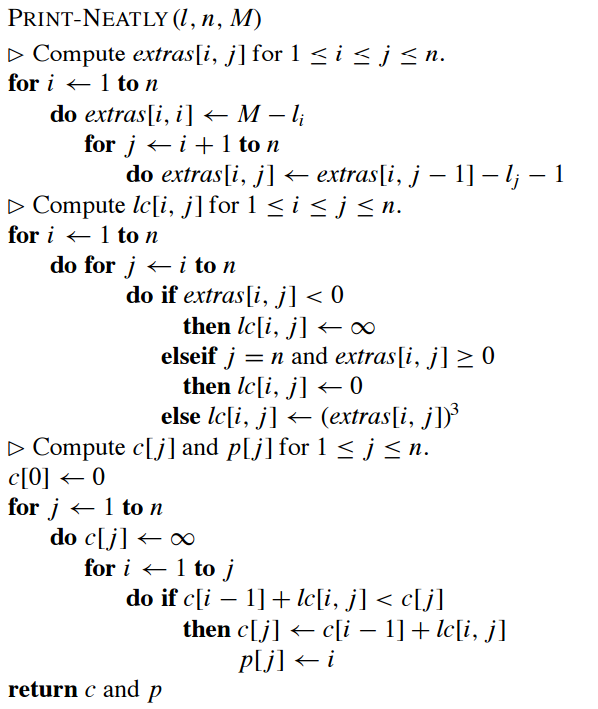
\includegraphics[width=0.65\textwidth]{q6-13-p1.png}
\end{align}

Quite clearly the time and space are $\Theta(n^2)$, but we can get both down to $\Theta(nM)$ (at most \ceil{M/2} words can fit on a line). The space can even further for $\Theta(n)$.

Here's how we print which words are on which line. The printed output of $\proc{Give-Lines}(p, j)$ is a sequence of triples $(k, i, j)$, indicating that words $i, \ldots , j$ are printed on line $k$. The return value is the line number $k$.

\begin{align}
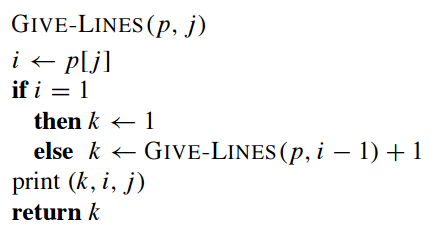
\includegraphics[width=0.5\textwidth]{q6-13-p2.png}
\end{align}

The initial call is $\proc{Give-Lines}(p, n)$. Since the value of $j$ decreases in each recursive call, $\proc{Give-Lines}$ takes a total of $O(n)$ time.\\[12pt]